\documentclass[conference]{IEEEtran}
\IEEEoverridecommandlockouts
% The preceding line is only needed to identify funding in the first footnote. If that is unneeded, please comment it out.
\usepackage{cite}
\usepackage{amsmath,amssymb,amsfonts}
\usepackage{algorithmic}
\usepackage{graphicx}
\usepackage{textcomp}
\usepackage{xcolor}
\def\BibTeX{{\rm B\kern-.05em{\sc i\kern-.025em b}\kern-.08em
    T\kern-.1667em\lower.7ex\hbox{E}\kern-.125emX}}
\begin{document}

\title{License Plate Reading}

\author{\IEEEauthorblockN{1\textsuperscript{st} Christopher Tomes}
\IEEEauthorblockA{\textit{Computer Science} \\
\textit{Cal Poly Pomona}\\
Anaheim, CA \\
tomes@cpp.edu}
\and
\IEEEauthorblockN{2\textsuperscript{nd} Jason Rowley}
\IEEEauthorblockA{\textit{Computer Science} \\
\textit{Cal Poly Pomona}\\
Torrance, CA \\
jrowley@cpp.edu}
\and
\IEEEauthorblockN{3\textsuperscript{rd} Anthony Seward}
\IEEEauthorblockA{\textit{Computer Science} \\
\textit{Cal Poly Pomona}\\
Montclair, CA \\
adseward@cpp.edu}
\and
\IEEEauthorblockN{4\textsuperscript{th} Joseph Luna}
\IEEEauthorblockA{\textit{Computer Science} \\
\textit{Cal Poly Pomona}\\
La Habra, CA \\
jmluna1@cpp.edu}
\and
\IEEEauthorblockN{5\textsuperscript{th} Mason Nash}
\IEEEauthorblockA{\textit{Computer Science} \\
\textit{Cal Poly Pomona}\\
Pomona, CA \\
mlnash@cpp.edu}
}

\maketitle

\begin{abstract}
% This document is a model and instructions for \LaTeX.
% This and the IEEEtran.cls file define the components of your paper [title, text, heads, etc.]. *CRITICAL: Do Not Use Symbols, Special Characters, Footnotes, 
% or Math in Paper Title or Abstract.
This paper evaluates a method for license plate detection using a camera to automatically detect license plates in case of accidents or law-breaking incidents. We aimed to use preprocessing techniques and machine learning to address these challenges, including masking the initial image to identify the location of the plates, using a multi-model pipeline, and segmenting the licence plate letters for individual classification. We planed to use the Vehicle-Rear dataset to train this multi-model pipeline. The proposed method aims to improve the accuracy of license plate detection, fortify against potential malicious actors, and minimize false positives and misclassifications. This research was conducted at California Polytechnic State University, Pomona over the course of two months, concluding on May 9, 2023.
\end{abstract}

\begin{IEEEkeywords}
convolutional network, u-net, neural network, pipeline, data science
\end{IEEEkeywords}

\section{Introduction}
License plate detection is useful to have when driving in the event someone gets in an accident or witnesses someone else breaking the law. This sort of problem sits squarely within the field of computer vision, which is itself situated within the field of machine learning. An ideal license plate detection system would be small and lightweight, able to be mounted on the dashboard of ordinary drivers to allow them to immediately be able to report any illegal driving activities or accidents of other drivers on the road. Any agent that could perform within this situation would need to be robust, for there is much variation it would experience from user to user. Different windshields would tint and refract light differently. Different dashboards would be at different heights, resulting in different video angles of the licence plates. 
\par
Our team recognized these difficulties, and realized that before tackling them it would be wise to first create a functional system for identifying plates within a more restrained scope of data. The Vehicle-Rear dataset contains a wealth of information about the vehicles and license plates in its hours of video footage. However, it is limited to the vantage point of a traffic camera. Despite this limitation, the data  was plenty to construct a working prototype  pipeline that can be refined for a wider dataset in future research. 

\section{Dataset}
The dataset we intend to use is the Vehicle-Rear dataset. This dataset "contains more than three hours of high-resolution videos, with accurate information about the make, model, color and year of nearly 3,000 vehicles, in addition to the position and identification of their license plates" [1]. We used the subset of this data with thorough class information. Each image is paired with a text file with the class information, including the following information:
\begin{itemize}
\item The number of Vehicles in the image
\item The coordinates of a bounding box around each vehicle
\item The type of vehicle, ex. Car
\item The characters of each license plate for each vehicle
\item the coordinates of a bounding box around each licence plate
\item the coordinates of a bounding box around each character of each plate
\end{itemize}
\par
This dataset has a few flaws that make training more difficult. First, the resolution is limited to 1920 \texttimes\ 1080 pixels, which means that once the  licence plate characters are isolated, they have a low resolution because they take up so little of the original frame. Next, because the images have varying numbers of vehicles, it is not simple to merely generate coordinates for bounding boxes. Third, the file format for the classes is not comma separated values, so extra code has to be written to parse the classes. Fourth, the amount of data in this set with the thorough labeling above is very limited, requiring extra preprocessing  to tweak the images to create new ones, thereby simulating a larger dataset.
\par
For training, we will test out several different ratios of testing and training data, and in order to evaluate it's real-world performance, we will also test the model on a separate set consisting of unlabeled data collected from a few different smartphones. This will allow us to determine whether our data augmentation is effectively facilitating the change in domain. In future research, we would like to fortify our models by introducing increased variation into our dataset so that the model can be deployed in a wider variety of situations and devices. Such variation could include camera shake. Camera shake could be simulated through preprocessing. In addition, having labeled footage from different angles would broaden our models' deployment potential. As it stands, this dataset is produced by a single high camera angle, and as a result the model will be more skilled at identifying plates from the vantage point of a traffic camera, but not, for example, a dashboard camera mounted behind a reflective windshield. In future research, we would like to produce and label more footage.

\section{Methodology}
\begin{figure}[h]
   \centering
   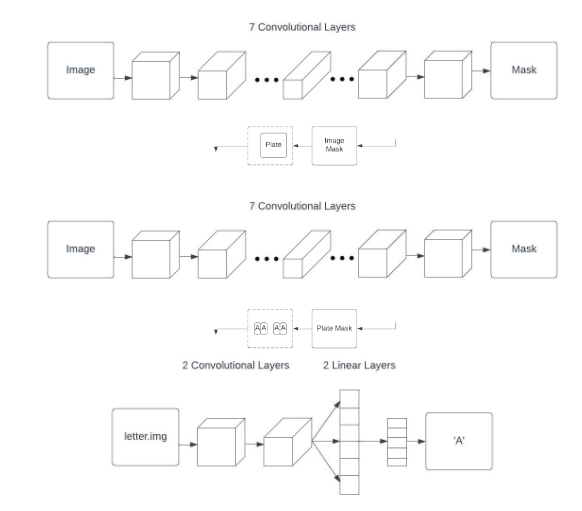
\includegraphics[width=0.5\textwidth]{layers.png}
   \caption{Diagram of full pipeline}
   \label{fig:image_label}
\end{figure}
The original planned methodology was to train several models on this dataset and compare their performance. As the project developed and the first models were being built, the team gained a better understanding of the complexity required from a pipeline with several models. The main hurdle is that the accuracy of each model affects the accuracy of later models. If the first model performs with poor accuracy, later models will also have poor accuracy. This is the classic idea in machine learning of garbage in, garbage out. Because of this challenge, and the restriction of the report's due date, the team decided to focus development toward refining the multi-model pipeline rather than developing several models. The adjusted and final goal of this project is to produce a robust pipeline that can identify with high accuracy the contents of several licence plates in a single image. Special care was put into preprocessing techniques, since they are key in cultivating the usability of data passing between models. For the preprocessing, and many of the models in our pipeline, the work Mr. Seward has done on the Cal Poly Pomona Ember UAV project proved invaluable. See Section V Related Works for more details on this project. 
\par
In this project, we used several 3rd party libraries. Numpy was used for data manipulation. OpenCV was used for image manipulation, especially in the pre and postprocessing steps. PyTorch and Torchvision was used to build the models. Matplotlib was useful for generating graphs of the models' performances for both the researcher's analysis and for the later presentation's audience.

\par
Before discussing the details of implementation, here is an overview of our training steps: 

\begin{itemize}
\item Apply Filters to the dataset to create a larger virtual dataset. For the rest of the steps, this virtual set is the dataset referred to.
\item Separate the dataset into training samples and test samples.
\item Create masked images from the coordinates of the licence plate bounding boxes provided by the class data.
\item Train a U-Net to produce images masked with respect to licence plate positions. The dataset's images are used for feature values. The images masked with respect to licence plate bounding boxes are used as class values.
\item Create cropped images of the licence plates from the coordinates of the licence plate bounding boxes provided by the class data.
\item Create masked images from the coordinates of the character bounding boxes provided by the class data.
\item Resize the plate images and masks to a standard resolution.
\item Train a U-Net to produce masks to segment each character so the characters can be processed separately in the next model. The cropped images of the licence plates are used as feature values. The images masked with respect to character position are used as class values.
\item Create cropped images of the licence plate characters from the coordinates of the character bounding boxes provided by the class data.
\item Resize the plate images and masks to a standard resolution.
\item Train a convolutional network to identify the characters. The cropped images of the characters are used for feature values. The classes for the characters are provided by the dataset.
\end{itemize}

 \par
 As the models were being trained, we also created the complete pipeline for them to cooperate to produce the final prediction: 
 
\begin{itemize}
\item Use the first U-Net to produce an image masked with respect to licence plate positions.
\item Use a Gaussian blur and threshold on the mask to clean noise from the prediction.
\item Generate bounding boxes around the processed masks.
\item Crop the image to the licence plate areas defined by the bounding boxes.
\item Perform an erosion operation on the cropped images to further separate the letters and make them easier to segment for the model.
\item Use the second U-Net on the crops generated by the previous steps to produce an image masked with respect to character positions.
\item Clean noise from the prediction, box, and crop using the same steps as above.
\item sharpen the cropped images to assist the third model with prediction
\item use a convolutional neural network to classify each image from the crop as an alphanumeric character
\item concatenate the string predictions to generate an overall prediction of the licence plate
\end{itemize}
\par
See Fig. 1 for a diagram of this pipeline

\par
The first month of research was spent understanding the dataset. This was a challenge because the file structure seemed convoluted at first, for reasons including nested zip files and inconsistent file types. By the end of this period of the research, we had largely grasped the structure of the data, and written a parsing function for extracting the class information from the file.
\par
Throughout the second month, we devoted ourselves to building the pipeline. For each model, the code for training and the code for pre-processing the training data were developed in parallel. As we discovered new quirks of each model, that information was immediately applied to the training data's prepossessing code.


\section{Results}
\begin{figure}[h]
   \centering
   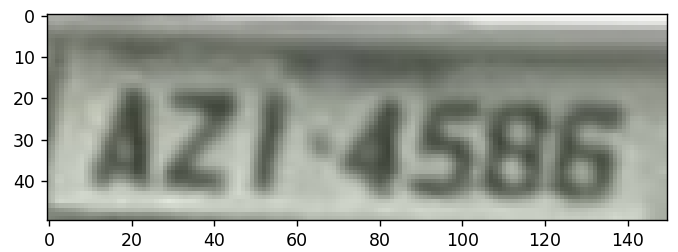
\includegraphics[width=0.5\textwidth]{plate.png}
   \caption{A plate cropped successfully by our first model}
   \label{fig:image_label}
\end{figure}
\begin{figure}[h]
   \centering
   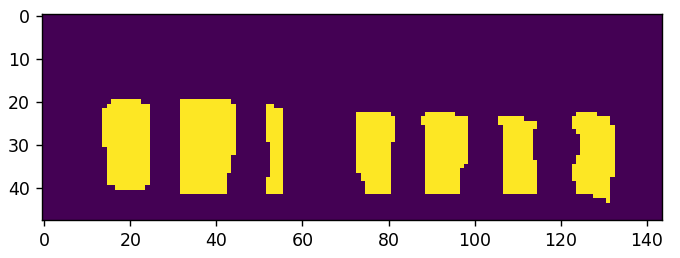
\includegraphics[width=0.5\textwidth]{charMask.png}
   \caption{Masks generated by our second model for the characters of Fig. 2}
   \label{fig:image_label}
\end{figure}
Now that the end of the research period has been reached, a full pipeline has been created. It takes in a JPEG, and results in a set of 7-character groups.
\par
The first performance metric used to evaluate the model is a partial accuracy. Specifically, the Levenshtein Distance is used to compare the predicted license plate number and the real one during testing. The Levenshtein Distance, intuitively, is the number of single-character substitutions, insertions, and deletions necessary to transform one string into another. For example, changing the string A4B6C into L3B6C would require A to be substituted with L and 4 to be substituted with 3. Therefore, the Levenshtein Distance would be 2. We consider a prediction partially correct if the Levenshtein Distance between the prediction and ground truth plate number is less than the length of the plate number minus 3. So if the plate number was 6 digits long, and the Levenshtein Distance between the prediction and ground truth was 2, then the prediction would be considered partially correct because 6 - 3 = 3 which is greater than 2. For our model, 37.5\% of the predictions are partially correct. As a baseline comparison, randomly predicting the license plate number results in only 1.97 x 1$0^{5}$ predictions being partially correct.
\par


\section{Related Work}
\par 
In Recent years there has been a growing interest in using deep learning techniques, such as Convolutional Neural Networks (CNN) for image recognition. Some related works implementing the structure proposed by “U-Net: Convolutional Networks for Biomedical Image Segmentation" biomedical recognition and wildfire detection. License Plate Recognition technology has evolved from simple optical character recognition to more advanced machine learning-based systems that can accurately recognize license plates in a variety of environments. In a study by Babu P. Mohan, the use of artificial intelligence in computer-aided diagnosis of gastrointestinal lesions was evaluated through convolutional neural networks (CNN). The meta-analysis conducted by the researchers demonstrated that CNN-based AI can be effectively used in the diagnosis of gastrointestinal neoplasia from endoscopic images, highlighting the potential of AI in medical diagnosis.
\par 
On the other hand, Bronco Ember is a nascent wildfire detection system that leverages edge computing capabilities, multi-spectral imaging, and artificial intelligence to significantly enhance the performance of small satellite remote sensing payloads. The project has developed a core hardware configuration that includes a SWIR InGaAs camera and a GPU-enabled single board computer. The system uses artificial intelligence for fire detection and analysis using computer vision and neural networks that can detect fires filling only a few pixels in each image. The neural network is trained to monitor the movement and spread of the fire, reducing the number of false positives detected.
\par
While LPR, Bio-Imaging, and wildfire detection are distinct, they all utilize similar artificial intelligence techniques to enhance their respective capabilities. These techniques have been shown to have significant potential in various applications, such as medical diagnosis and environmental monitoring. The studies conducted by Babu P. Mohan and the Bronco Ember project demonstrate how AI can be effectively used in diverse fields and highlight the potential for further research in these areas.
\par
BioMed Recog:
https://www.ncbi.nlm.nih.gov/pmc/articles\linebreak[0]/PMC7581460/pdf/10-1055-a-1236-3007.pdf
Original Presentation
https://arxiv.org/pdf/1505.04597.pdf
Work by Ember wild fire detection:
"https://digitalcommons.usu.edu/cgi/viewcontent.cgi?article=5\linebreak[0]259\&context=smallsat"



\section{Conclusion}
This project really highlights the importance of preprocessing and postprocessing for a machine learning task. So many steps in the pipeline meant a massive amount of hyperparameters, from the net architectures to the types and specifications of the processing techniques used between the models. The biggest performance increases came with changes to preprocessing and postprocessing techniques. Making the task easier for the model proved to be more effective than making the model more well suited for the task. It was also much easier to and faster to predict and confirm whether something would have a positive or negative impact when applying filters before and/or after the model than changing the model architecture and retraining. A specific example of this phenomenon is when blurring and thresholding was applied to the masks. No matter what changes were made to the model, its predictions were extremely unreliable before the outputs were blurred and thresholded to remove noise. That change was the single greatest This is not to say that tuning the model is not important. In this case where the output of one model is processed to be the input of the next, any increase of accuracy is important; however, effects of changes to model architecture were felt much greater after the images were processed prior to evaluation by the model.

%\section{Prepare Your Paper Before Styling}
%Before you begin to format your paper, first write and save the content as a 
%separate text file. Complete all content and organizational editing before 
%formatting. Please note sections \ref{AA}--\ref{SCM} below for more information on 
%proofreading, spelling and grammar.

%Keep your text and graphic files separate until after the text has been 
%formatted and styled. Do not number text heads---{\LaTeX} will do that 
%for you.

%\subsection{Abbreviations and Acronyms}\label{AA}
%Define abbreviations and acronyms the first time they are used in the text, 
%even after they have been defined in the abstract. Abbreviations such as 
%IEEE, SI, MKS, CGS, ac, dc, and rms do not have to be defined. Do not use 
%abbreviations in the title or heads unless they are unavoidable.

%\subsection{Units}
%\begin{itemize}
%\item Use either SI (MKS) or CGS as primary units. (SI units are encouraged.) English units may be used as secondary units (in parentheses). An exception would %be the use of English units as identifiers in trade, such as ``3.5-inch disk drive''.
%\item Avoid combining SI and CGS units, such as current in amperes and magnetic field in oersteds. This often leads to confusion because equations do not balance %dimensionally. If you must use mixed units, clearly state the units for each quantity that you use in an equation.
%\item Do not mix complete spellings and abbreviations of units: ``Wb/m\textsuperscript{2}'' or ``webers per square meter'', not ``webers/m\textsuperscript{2}''. %Spell out units when they appear in text: ``. . . a few henries'', not ``. . . a few H''.
%\item Use a zero before decimal points: ``0.25'', not ``.25''. Use ``cm\textsuperscript{3}'', not ``cc''.)
%\end{itemize}

%\subsection{Equations}
%Number equations consecutively. To make your 
%equations more compact, you may use the solidus (~/~), the exp function, or 
%appropriate exponents. Italicize Roman symbols for quantities and variables, 
%but not Greek symbols. Use a long dash rather than a hyphen for a minus 
%sign. Punctuate equations with commas or periods when they are part of a 
%sentence, as in:
%\begin{equation}
%a+b=\gamma\label{eq}
%\end{equation}

%Be sure that the 
%symbols in your equation have been defined before or immediately following 
%the equation. Use ``\eqref{eq}'', not ``Eq.~\eqref{eq}'' or ``equation \eqref{eq}'', except at 
%the beginning of a sentence: ``Equation \eqref{eq} is . . .''

%\subsection{\LaTeX-Specific Advice}

%Please use ``soft'' (e.g., \verb|\eqref{Eq}|) cross references instead
%of ``hard'' references (e.g., \verb|(1)|). That will make it possible
%to combine sections, add equations, or change the order of figures or
%citations without having to go through the file line by line.

%Please don't use the \verb|{eqnarray}| equation environment. Use
%\verb|{align}| or \verb|{IEEEeqnarray}| instead. The \verb|{eqnarray}|
%environment leaves unsightly spaces around relation symbols.

%Please note that the \verb|{subequations}| environment in {\LaTeX}
%will increment the main equation counter even when there are no
%equation numbers displayed. If you forget that, you might write an
%article in which the equation numbers skip from (17) to (20), causing
%the copy editors to wonder if you've discovered a new method of
%counting.

% {\BibTeX} does not work by magic. It doesn't get the bibliographic
% data from thin air but from .bib files. If you use {\BibTeX} to produce a
% bibliography you must send the .bib files. 

% {\LaTeX} can't read your mind. If you assign the same label to a
% subsubsection and a table, you might find that Table I has been cross
% referenced as Table IV-B3. 

% {\LaTeX} does not have precognitive abilities. If you put a
% \verb|\label| command before the command that updates the counter it's
% supposed to be using, the label will pick up the last counter to be
% cross referenced instead. In particular, a \verb|\label| command
% should not go before the caption of a figure or a table.

% Do not use \verb|\nonumber| inside the \verb|{array}| environment. It
% will not stop equation numbers inside \verb|{array}| (there won't be
% any anyway) and it might stop a wanted equation number in the
% surrounding equation.

% \subsection{Some Common Mistakes}\label{SCM}
% \begin{itemize}
% \item The word ``data'' is plural, not singular.
% \item The subscript for the permeability of vacuum $\mu_{0}$, and other common scientific constants, is zero with subscript formatting, not a lowercase letter ``o''.
% \item In American English, commas, semicolons, periods, question and exclamation marks are located within quotation marks only when a complete thought or name is cited, such as a title or full quotation. When quotation marks are used, instead of a bold or italic typeface, to highlight a word or phrase, punctuation should appear outside of the quotation marks. A parenthetical phrase or statement at the end of a sentence is punctuated outside of the closing parenthesis (like this). (A parenthetical sentence is punctuated within the parentheses.)
% \item A graph within a graph is an ``inset'', not an ``insert''. The word alternatively is preferred to the word ``alternately'' (unless you really mean something that alternates).
% \item Do not use the word ``essentially'' to mean ``approximately'' or ``effectively''.
% \item In your paper title, if the words ``that uses'' can accurately replace the word ``using'', capitalize the ``u''; if not, keep using lower-cased.
% \item Be aware of the different meanings of the homophones ``affect'' and ``effect'', ``complement'' and ``compliment'', ``discreet'' and ``discrete'', ``principal'' and ``principle''.
% \item Do not confuse ``imply'' and ``infer''.
% \item The prefix ``non'' is not a word; it should be joined to the word it modifies, usually without a hyphen.
% \item There is no period after the ``et'' in the Latin abbreviation ``et al.''.
% \item The abbreviation ``i.e.'' means ``that is'', and the abbreviation ``e.g.'' means ``for example''.
% \end{itemize}
% An excellent style manual for science writers is \cite{b7}.

% \subsection{Figures and Tables}
% \paragraph{Positioning Figures and Tables} Place figures and tables at the top and 
% bottom of columns. Avoid placing them in the middle of columns. Large 
% figures and tables may span across both columns. Figure captions should be 
% below the figures; table heads should appear above the tables. Insert 
% figures and tables after they are cited in the text. Use the abbreviation 
% ``Fig.~\ref{fig}'', even at the beginning of a sentence.

% \begin{table}[htbp]
% \caption{Table Type Styles}
% \begin{center}
% \begin{tabular}{|c|c|c|c|}
% \hline
% \textbf{Table}&\multicolumn{3}{|c|}{\textbf{Table Column Head}} \\
% \cline{2-4} 
% \textbf{Head} & \textbf{\textit{Table column subhead}}& \textbf{\textit{Subhead}}& \textbf{\textit{Subhead}} \\
% \hline
% copy& More table copy$^{\mathrm{a}}$& &  \\
% \hline
% \multicolumn{4}{l}{$^{\mathrm{a}}$Sample of a Table footnote.}
% \end{tabular}
% \label{tab1}
% \end{center}
% \end{table}

% \begin{figure}[htbp]
% \centerline{\includegraphics{fig1.png}}
% \caption{Example of a figure caption.}
% \label{fig}
% \end{figure}

% Figure Labels: Use 8 point Times New Roman for Figure labels. Use words 
% rather than symbols or abbreviations when writing Figure axis labels to 
% avoid confusing the reader. As an example, write the quantity 
% ``Magnetization'', or ``Magnetization, M'', not just ``M''. If including 
% units in the label, present them within parentheses. Do not label axes only 
% with units. In the example, write ``Magnetization (A/m)'' or ``Magnetization 
% \{A[m(1)]\}'', not just ``A/m''. Do not label axes with a ratio of 
% quantities and units. For example, write ``Temperature (K)'', not 
% ``Temperature/K''.

% \section*{References}

% Please number citations consecutively within brackets \cite{b1}. The 
% sentence punctuation follows the bracket \cite{b2}. Refer simply to the reference 
% number, as in \cite{b3}---do not use ``Ref. \cite{b3}'' or ``reference \cite{b3}'' except at 
% the beginning of a sentence: ``Reference \cite{b3} was the first $\ldots$''

% Number footnotes separately in superscripts. Place the actual footnote at 
% the bottom of the column in which it was cited. Do not put footnotes in the 
% abstract or reference list. Use letters for table footnotes.

% Unless there are six authors or more give all authors' names; do not use 
% ``et al.''. Papers that have not been published, even if they have been 
% submitted for publication, should be cited as ``unpublished'' \cite{b4}. Papers 
% that have been accepted for publication should be cited as ``in press'' \cite{b5}. 
% Capitalize only the first word in a paper title, except for proper nouns and 
% element symbols.

% For papers published in translation journals, please give the English 
% citation first, followed by the original foreign-language citation \cite{b6}.

\begin{thebibliography}{00}
\bibitem{b1} I. O. de Oliveira, R. Laroca, D. Menotti, K. V. O. Fonseca, R. Minetto, “Vehicle-Rear: A New Dataset to Explore Feature Fusion for Vehicle Identification Using Convolutional Neural Networks,” IEEE Access, vol. 9, pp. 101065-101077, 2021.
% \bibitem{b1} G. Eason, B. Noble, and I. N. Sneddon, ``On certain integrals of Lipschitz-Hankel type involving products of Bessel functions,'' Phil. Trans. Roy. Soc. London, vol. A247, pp. 529--551, April 1955.
% \bibitem{b2} J. Clerk Maxwell, A Treatise on Electricity and Magnetism, 3rd ed., vol. 2. Oxford: Clarendon, 1892, pp.68--73.
% \bibitem{b3} I. S. Jacobs and C. P. Bean, ``Fine particles, thin films and exchange anisotropy,'' in Magnetism, vol. III, G. T. Rado and H. Suhl, Eds. New York: Academic, 1963, pp. 271--350.
% \bibitem{b4} K. Elissa, ``Title of paper if known,'' unpublished.
% \bibitem{b5} R. Nicole, ``Title of paper with only first word capitalized,'' J. Name Stand. Abbrev., in press.
% \bibitem{b6} Y. Yorozu, M. Hirano, K. Oka, and Y. Tagawa, ``Electron spectroscopy studies on magneto-optical media and plastic substrate interface,'' IEEE Transl. J. Magn. Japan, vol. 2, pp. 740--741, August 1987 [Digests 9th Annual Conf. Magnetics Japan, p. 301, 1982].
% \bibitem{b7} M. Young, The Technical Writer's Handbook. Mill Valley, CA: University Science, 1989.
\end{thebibliography}
% \vspace{12pt}
% \color{red}
% IEEE conference templates contain guidance text for composing and formatting conference papers. Please ensure that all template text is removed from your conference paper prior to submission to the conference. Failure to remove the template text from your paper may result in your paper not being published.

\end{document}
